\documentclass [a4paper,11pt]{article}
\usepackage{amssymb}
\usepackage{amsthm}
\usepackage[intlimits]{amsmath}
\usepackage[polish]{babel}
\usepackage[utf8]{inputenc}
\usepackage[T1]{fontenc}
\frenchspacing
\usepackage{indentfirst}
\usepackage{graphicx}
\usepackage{subfig}
\usepackage{mathptmx}
\usepackage{geometry}
\usepackage{wrapfig}
\usepackage{enumitem}

\title{Moduł Younga}
\author{Pęcak Tomasz, Bielech Maciej}

\begin{document}
	
	\renewcommand*{\figurename}{Tabela} 
	\newgeometry{tmargin=2cm, bmargin=2cm, lmargin=2cm, rmargin=2cm}
	
	\linespread{1.5}
	\selectfont

	\begin{table}[]
		\centering
		\begin{tabular}{lllllll}
			\cline{1-6}
			\multicolumn{1}{|c|}{\begin{tabular}[c]{@{}c@{}}EAiIB\\ Informatyka\end{tabular}} & \multicolumn{2}{l|}{\begin{tabular}[c]{@{}l@{}}Pęcak Tomasz\\ Bielech Maciej\end{tabular}} & \multicolumn{1}{c|}{\begin{tabular}[c]{@{}c@{}}Rok\\ II\end{tabular}} & \multicolumn{1}{c|}{\begin{tabular}[c]{@{}c@{}}Grupa\\ 3a\end{tabular}} & \multicolumn{1}{c|}{\begin{tabular}[c]{@{}c@{}}Zespół\\ II\end{tabular}} &  \\ \cline{1-6}
			\multicolumn{1}{|c|}{\begin{tabular}[c]{@{}c@{}}Pracownia\\ FIZYCZNA\\ WFiIS AGH\end{tabular}} & \multicolumn{4}{l|}{\begin{tabular}[c]{@{}l@{}}Temat:\\ \textbf{Moduł Younga} \end{tabular}} & 
			\multicolumn{1}{l|}{\begin{tabular}[c]{@{}l@{}}nr ćwiczenia:\\ 11\end{tabular}} &  \\ \cline{1-6}
			\multicolumn{1}{|l|}{\begin{tabular}[c]{@{}c@{}}Data wykonania:\\ 21.10.2017\end{tabular}} & \multicolumn{1}{c|}{\begin{tabular}[c]{@{}c@{}}Data oddania:\\ 24.10.2017\end{tabular}} & \multicolumn{1}{l|}{\begin{tabular}[c]{@{}l@{}}Zwrot do poprawki:\\ \phantom{data poprawki}\end{tabular}} & \multicolumn{1}{l|}{\begin{tabular}[c]{@{}l@{}}Data oddania:\\  \phantom{data oddania}\end{tabular}} & \multicolumn{1}{l|}{\begin{tabular}[c]{@{}l@{}}Data zaliczenia:\\  \phantom{data zaliczenia}\end{tabular}} & \multicolumn{1}{l|}{\begin{tabular}[c]{@{}l@{}}OCENA:\\ \phantom{ocena}\end{tabular}} &  \\ \cline{1-6} 
		\end{tabular}
	\end{table}
	 \hspace{5mm}

	\section{Wstęp}
	Celem ćwiczenia było wyznaczenie wartości modułu Younga poprzez pomiar wydłużenia drutu z mosiądzu i stali. Aby wyznaczyć moduł Younga należało obciążać druty coraz większą siłą.
	
	Moduł Younga ($E$) nazywany współczynnikiem sprężystości podłużnej jest to wielkość określająca własności sprężyste ciała stałego, charakteryzująca podatność materiału na odkształcenia podłużne przy rozciąganiu, ściskaniu, czy zginaniu.
	
	W prawie Hooke’a (\ref{eq:prawohooka}) moduł Younga stanowi współczynnik proporcjonalności między naprężeniem i odkształceniem:
	\begin{equation}
	\label{eq:prawohooka}
	\sigma = E \epsilon.
	\end{equation}
	
	Wartość modułu Younga wyznaczana jest doświadczalnie. Nazwa pochodzi od nazwiska Thomasa Younga. Jednostką modułu Younga jest pascal $\left[ \text{Pa} \right]$.
	\begin{equation}
	\label{eq:modulyounga}
		E = \frac{F l}{S \Delta l}
	\end{equation}
	\begin{equation}
	\label{eq:sila}
	F = mg
	\end{equation}
	\begin{equation}
	\label{eq:powprzekroju}
	S = \frac{ \pi d^2 }{4}
	\end{equation}
	Przekształcając wzór na moduł Younga (\ref{eq:modulyounga}), korzystając z wzorów na siłę (\ref{eq:sila}) i powierzchnię przekroju druta (\ref{eq:powprzekroju}) otrzymujemy następującą zależność:
	\begin{equation}
		\label{eq:wzorroboczy}
		E = \frac{4mgl}{\pi d^2 \Delta l} \text{.}
	\end{equation}
	
	\vspace{1em}
	\noindent
	W celu oszacowania modułu Younga skorzystaliśmy z następujących metod:
	\begin{itemize}
		\item Wykonywanie wykresów	
		\item Regresja liniowa
		\item Linearyzacja nieliniowych zależności funkcyjnych
		\item Wykorzystanie współczynnika prostej do obliczeń
	\end{itemize}
	
	\section{Wykonanie ćwiczenia}
	Ćwiczenie wykonywaliśmy dla drutów: mosiężnego i stalowego. Dla każdego z nich wykonaliśmy nastepujące czynności:
	\begin{itemize}
		\item W pierwszym kroku dokonaliśmy pomiaru długości drutu przy użyciu przymiaru milimetrowego z~dokładnością 1 mm.
		
		\item Następnie po wcześniejszym obciążeniu drutu masą około 2kg zmierzyliśmy średnicę drutu za pomocą śruby mikrometrycznej z~dokładnością 0,01 mm. Pomiaru tego dokonaliśmy w pięciu miejscach, aby sprawdzić czy drut ma stałą średnicę.
		
		\item Kolejnym krokiem było opróżnienie szalki z odważników i wyzerowanie czujnika mikrometrycznego.
		
		\item Po tym obciążaliśmy szalkę przez dokładanie kolejnych odważników notując w tabeli sumaryczną masę odważników i wynikające wydłużenie drutu. Odważniki ważyliśmy na wadze o dokładności do 1 g. Pomiary wykonywaliśmy przy dokładaniu odważników ($\uparrow $) i przy ich zdejmowaniu ($\downarrow $), dla lepszej dokładności.
		
		\item Wykonując ćwiczenie dbaliśmy o to, aby odkształcenie drutu było sprężyste, gdyż po przekroczeniu granicy sprężystości drut uległ by odkształceniu nieodwracalnemu, co niekorzystnie wpłynęłoby na wyniki obliczeń.
		
		\item Wartosci odczytane z czujnika przenieśliśmy do tabel: (\ref{fig:tebmosiadz}, \ref{fig:tebmosiadz2}) dla mosiądzu i (\ref{fig:tabstal}) dla stali. Dla mosiądzu wykonaliśmy dwie serie pomiarów ze względu na błąd systematyczny, o którym domyślaliśmy się wykonując pomiary pierwszej serii (więcej w sekcji \ref{sec:opr}).
	
	\begin{figure}[!h]
		\centering
		\caption{Pomiary dla drutu mosiężnego}
		%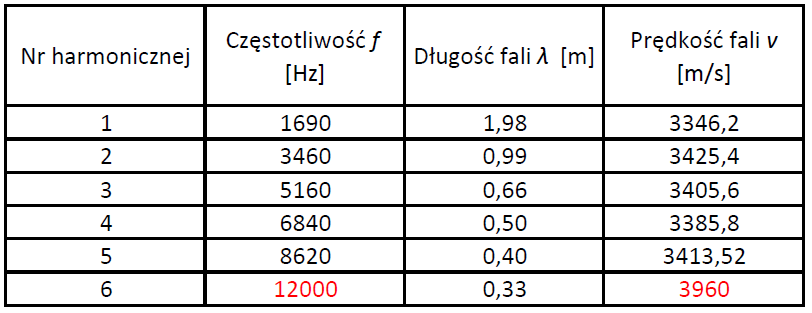
\includegraphics[width=0.7\textwidth]{tabmosiadz}
		\label{fig:tebmosiadz}
	\end{figure}
	
	\begin{figure}[!h]
		\centering
		\caption{Druga seria pomiarów dla drutu mosiężnego}
		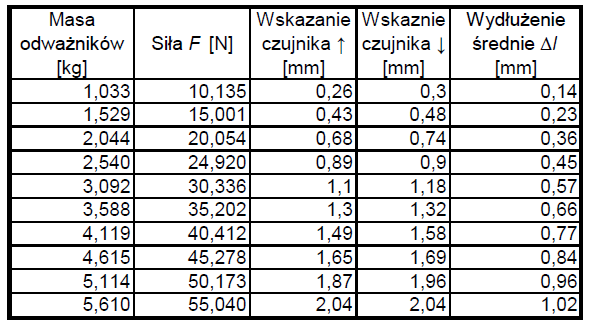
\includegraphics[width=0.7\textwidth]{tabmosiadz2}
		\label{fig:tebmosiadz2}
	\end{figure}
	
	\begin{figure}[!h]
		\centering
		\caption{Pomiary dla drutu stalowego}
		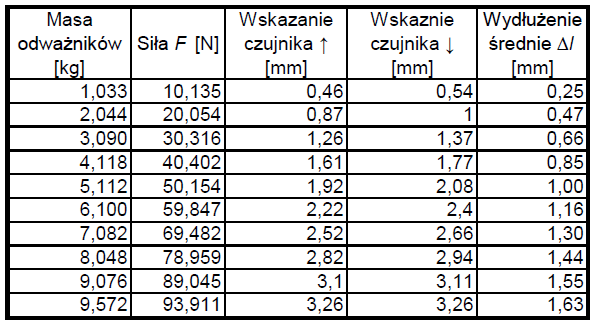
\includegraphics[width=0.7\textwidth]{tabstal}
		\label{fig:tabstal}
	\end{figure}
		
	\end{itemize}

	\renewcommand*{\figurename}{Wykres} 
	\setcounter{figure}{0}
	
	\section{Opracowanie danych pomiarowych}\label{sec:opr}
	\begin{enumerate}[label=\alph*)]
		\item Ocena niepewności pomiaru długości drutu.
		
		Pomiaru długości drutu dokonywaliśmy przymiarem milimetrowym z dokładnością do 1 mm. Jednak ze względu na odległość przymiaru od drutu przyjmujemy niepewność pomiaru typu B większą od dokładności przyrządu pomiarowego: $u(l) = 2 \text{ mm}$.
		
		\item Ocena niepewności pomiaru wydłużenia.
		
		Pomiaru wydłużenia dokonywaliśmy czujnikiem mikrometrycznego z dokładnością do 0,01 mm. Przyjmujemy więc niepewność pomiaru typu B równą dokładności przyrządu pomiarowego: $u(\Delta l) = 0,01 \text{ mm}$.
		
		\item Ocena niepewności pomiaru średnicy drutu.
		
		Pomiaru średnicy drutu dokonywaliśmy śrubą mikrometryczną z dokładnością do 0,01 mm. Przyjmujemy więc niepewność pomiaru typu B równą dokładności przyrządu pomiarowego: $u(d) = 0,01 \text{ mm}$.
		
		\item Ocena niepewności pomiaru masy ciężarków.
		
		Pomiaru masy dokonywaliśmy wagą elektroniczną z dokładnością do 1 g. Przyjmujemy więc niepewność pomiaru typu B równą: $u(m) = 1 \text{ g}$ dla każdego ciężarka.
	\end{enumerate}
	
	\subsection{Opracowanie danych dla drutu mosiężnego.}
	
	\begin{figure}[!h]
		\centering
		%\includegraphics[width=0.8\textwidth]{wykmosiadz}
		\caption{Wykres regresji liniowej dla pomiaru modułu Younga mosiądzu.}
		\label{fig:wykmosiadz}
	\end{figure}

	\begin{enumerate}[label=\alph*)]
		\item Analiza błędów
		
		Nie stwierdziliśmy wystąpienia błędów grubych, gdyż na wykresie (\ref{fig:wykmosiadz}) nie zauważamy pomiarów odstających.
		
		\item Prawo przenoszenia niepewności.
		
		Obliczając niepewność złożoną (\ref{eq:niepewnosczlozonamosiadz}) oraz rozszerzoną (\ref{eq:rozszerzonamosiadz}) dochodzimy do wyników: 
		\begin{equation}
		\label{eq:niepewnosczlozonamosiadz}
		u_c(E) = \sqrt{ \left[ \frac{4mg}{\pi d^2\Delta l}u(l) \right]^2 + \left[ -\frac{8mgl}{\pi d^3\Delta l}u(d) \right]^2 + \left[ -\frac{4mgl}{\pi d^2\Delta l^2}u(\Delta l) \right]^2 + \left[ \frac{4gl}{\pi d^2\Delta l}u(m) \right]^2}
		\end{equation}
		$$ u_c(E) = 0,XXX \text{ GPa,} $$
		\begin{equation}
		\label{eq:rozszerzonamosiadz}
		U(E) = k\cdot u_c(E) = 2 \cdot 0,XXX \text{ }\mathrm{GPa} = 0,XXX \text{ }\mathrm{GPa}
		\end{equation}
		
		Niepewość względna złożona jest równa:
		\begin{equation}
		\label{eq:niepewnosczlozonawzglmosiadz}
		\frac{u_c(E)}{E} = \sqrt{ \left[ \frac{u(l)}{l} \right]^2 + \left[ -2\frac{u(d)}{d} \right]^2 + \left[ -\frac{u(\Delta l)}{\Delta l} \right]^2 + \left[ \frac{u(m)}{m} \right]^2}
		\end{equation}
		$$ \frac{u_c(E)}{E} = 0,XX\% $$
		
		\item Zastosowanie niepewności rozszerzonej do oceny zgodności z wartością dokładną.
		
		Różnica pomiedzy obliczoną wartością modułu Younga, a wartością tabelaryczną wynosi:
		\begin{equation}
		\label{eq:roznicamosiadz}
		|E - E_0| = \left|X,XXX \text{ }\mathrm{GPa} - X,XXX \text{ }\mathrm{GPa}\right| = X,XXX \text{ }\mathrm{GPa}.
		\end{equation}
		
		Niepewność rozszerzona wyniku jest mniejsza od modułu różnicy pomiędzy obliczoną wartością przyspieszenia, a wartością tabelaryczną. Nie możemy więc uznać, że policzona wartość modułu Younga jest zgodna z wartością tabelaryczną w zakresie wyznaczonej niepewności. Wyniki pomiarów w przybliżeniu liniowe i niezgodny wynik mogą świadczyć o błędzie systematycznym. Było to złe wyzerowanie czujnika, dlatego każdy z pomiarów wskazuje niższą wartość wydłużenia drutu niż spodziewana. Błąd ten zauważyliśmy podczas wykonywania pomiarów, dlatego wykonaliśmy kolejną serie pomiarów dla drutu mosiężnego.
		
	\end{enumerate}

	\subsection{Opracowanie danych dla drutu mosiężnego. Wyniki drugiej serii pomiarów}
	
	\begin{figure}[!h]
		\centering
		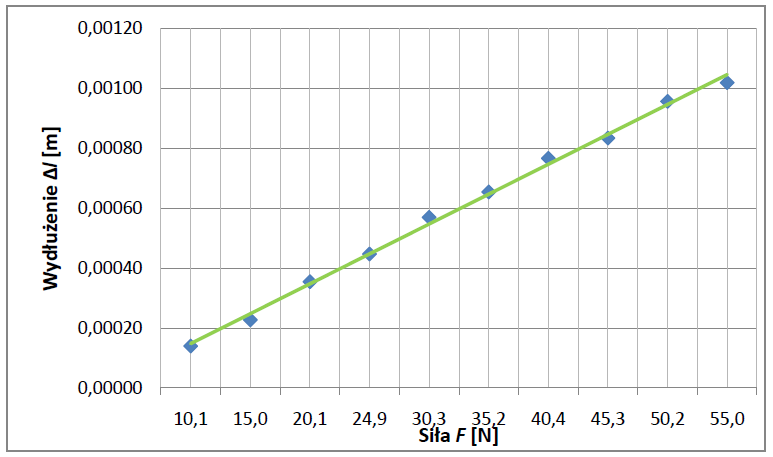
\includegraphics[width=0.8\textwidth]{wykmosiadz2}
		\caption{Wykres regresji liniowej dla drugiej serii pomiaru modułu Younga mosiądzu.}
		\label{fig:wykmosiadz2}
	\end{figure}
	
	\begin{enumerate}[label=\alph*)]
		\item Analiza błędów
		
		Nie stwierdziliśmy wystąpienia błędów grubych, gdyż na wykresie (\ref{fig:wykmosiadz2}) nie zauważamy pomiarów odstających.
		
		\item Prawo przenoszenia niepewności.
		
		Obliczając niepewność złożoną (\ref{eq:niepewnosczlozonamosiadz2}) oraz rozszerzoną (\ref{eq:rozszerzonamosiadz2}) dochodzimy do wyników: 
		\begin{equation}
		\label{eq:niepewnosczlozonamosiadz2}
		u_c(E) = \sqrt{ \left[ \frac{4mg}{\pi d^2\Delta l}u(l) \right]^2 + \left[ -\frac{8mgl}{\pi d^3\Delta l}u(d) \right]^2 + \left[ -\frac{4mgl}{\pi d^2\Delta l^2}u(\Delta l) \right]^2 + \left[ \frac{4gl}{\pi d^2\Delta l}u(m) \right]^2}
		\end{equation}
		$$ u_c(E) = 0,XXX \text{ GPa,} $$
		\begin{equation}
		\label{eq:rozszerzonamosiadz2}
		U(E) = k\cdot u_c(E) = 2 \cdot 0,XXX \text{ }\mathrm{GPa} = 0,XXX \text{ }\mathrm{GPa}
		\end{equation}
		
		Niepewość względna złożona jest równa:
		\begin{equation}
		\label{eq:niepewnosczlozonawzglmosiadz2}
		\frac{u_c(E)}{E} = \sqrt{ \left[ \frac{u(l)}{l} \right]^2 + \left[ -2\frac{u(d)}{d} \right]^2 + \left[ -\frac{u(\Delta l)}{\Delta l} \right]^2 + \left[ \frac{u(m)}{m} \right]^2}
		\end{equation}
		$$ \frac{u_c(E)}{E} = 0,XX\% $$
		
		\item Zastosowanie niepewności rozszerzonej do oceny zgodności z wartością dokładną.
		
		Różnica pomiedzy obliczoną wartością modułu Younga, a wartością tabelaryczną wynosi:
		\begin{equation}
		\label{eq:roznicamosiadz2}
		|E - E_0| = \left|X,XXX \text{ }\mathrm{GPa} - X,XXX \text{ }\mathrm{GPa}\right| = X,XXX \text{ }\mathrm{GPa}.
		\end{equation}
		
		Wyniki drugiej serii pomiarów dla drutu mosiężnego potwierdziły nasze przypuszczenia odnośnie złego wyzerowania czujnika. Tym razem niepewność rozszerzona wyniku jest większa od modułu różnicy pomiędzy obliczoną wartością modułu Younga, a wartością tabelaryczną. Uznajemy więc, że policzona wartość modułu Younga jest zgodna z wartością tabelaryczną w zakresie wyznaczonej niepewności.
		
	\end{enumerate}

	\subsection{Opracowanie danych dla drutu stalowego.}
	\begin{figure}[!h]
		\centering
		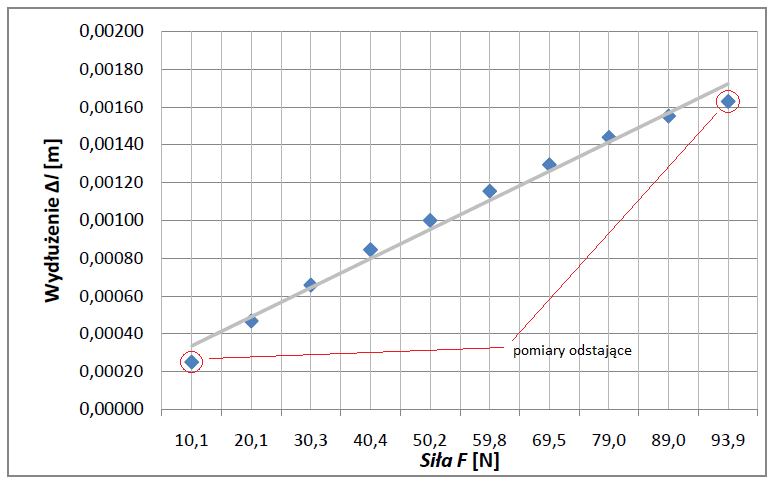
\includegraphics[width=0.8\textwidth]{wykstal}
		\caption{Wykres regresji liniowej dla pomiaru modułu Younga stali.}
		\label{fig:wykstal}
	\end{figure}
	
	\begin{enumerate}[label=\alph*)]
		\item Analiza błędów
		
		Stwierdziliśmy wystąpienie dwóch błędów grubych. Błędy te zaznaczylismy na wykresie (\ref{fig:wykstal}) jako pomiary odstające. Błędy te mogły zostać spowodowane niedokładnym wyzerowaniem czujnika, wygięciami druta lub błędnym odczytem pomiaru z czujnika.
		
		\item Prawo przenoszenia niepewności.
		
		Obliczając niepewność złożoną (\ref{eq:niepewnosczlozonastal}) oraz rozszerzoną (\ref{eq:rozszerzonastal}) dochodzimy do wyników: 
		\begin{equation}
		\label{eq:niepewnosczlozonastal}
		u_c(E) = \sqrt{ \left[ \frac{4mg}{\pi d^2\Delta l}u(l) \right]^2 + \left[ -\frac{8mgl}{\pi d^3\Delta l}u(d) \right]^2 + \left[ -\frac{4mgl}{\pi d^2\Delta l^2}u(\Delta l) \right]^2 + \left[ \frac{4gl}{\pi d^2\Delta l}u(m) \right]^2}
		\end{equation}
		$$ u_c(E) = 0,XXX \text{ GPa,} $$
		\begin{equation}
		\label{eq:rozszerzonastal}
		U(E) = k\cdot u_c(E) = 2 \cdot 0,XXX \text{ }\mathrm{GPa} = 0,XXX \text{ }\mathrm{GPa}
		\end{equation}
		
		Niepewość względna złożona jest równa:
		\begin{equation}
		\label{eq:niepewnosczlozonawzglstal}
		\frac{u_c(E)}{E} = \sqrt{ \left[ \frac{u(l)}{l} \right]^2 + \left[ -2\frac{u(d)}{d} \right]^2 + \left[ -\frac{u(\Delta l)}{\Delta l} \right]^2 + \left[ \frac{u(m)}{m} \right]^2}
		\end{equation}
		$$ \frac{u_c(E)}{E} = 0,XX\% $$
		
		\item Zastosowanie niepewności rozszerzonej do oceny zgodności z wartością dokładną.
		
		Różnica pomiedzy obliczoną wartością modułu Younga, a wartością tabelaryczną wynosi:
		\begin{equation}
		\label{eq:roznicastal}
		|E - E_0| = \left|X,XXX \text{ }\mathrm{GPa} - X,XXX \text{ }\mathrm{GPa}\right| = X,XXX \text{ }\mathrm{GPa}.
		\end{equation}
		
		Niepewność rozszerzona wyniku jest większa od modułu różnicy pomiędzy obliczoną wartością przyspieszenia, a wartością tabelaryczną. Uznajemy więc, że policzona wartość modułu Younga jest zgodna z wartością tabelaryczną w zakresie wyznaczonej niepewności.
		
	\end{enumerate}
	
	
	
	\section{Podsumowanie}
	
	\begin{center}
		\begin{tabular}{|c|c|c|c|c|c|}
			\hline Opis wielkości & Wartość tablicowa $\left[ \text{GPa} \right]$ & $E \left[ \text{GPa} \right]$ & $u(E) \left[ \text{GPa} \right]$ & $U(E) \left[ \text{GPa} \right]$ & $ \frac{u(E)}{E} $\\
			\hline Pomiary drutu mosiężnego & Tab & 9,872 & 0,064  & 0,128 & 0,7 \% \\ 
			\hline Pomiary drutu stalowego & Tab & 9,796  & 0,098  & 0,196 &  1 \%\\ 
			\hline 
		\end{tabular} 
	\end{center}

\end{document}